%versi 2 (8-10-2016)
\chapter{Landasan Teori}
\label{chap:teori}

\section{Skripsi}
\label{sec:skripsi} 
 
\subsection{Pengertian Permainan Snake}
\textit{Snake} merupakan permainan mengendalikan ular untuk mendapatkan makanan yang terdapat pada labirin. Dalam permainan ini, pemain mengendalikan ular untuk mendapatkan makanan sebanyak-banyaknya. Setiap ular memakan makanan, maka skor akan bertambah 1 poin dan tubuh ular akan bertambah panjang. Biasanya makanan hanya ada 1 saja pada sebuah labirin. Ketika makanan itu sudah termakan oleh ular, makanan tersebut akan ditempatkan secara acak. Ular dapat bergerak ke atas, bawah, kiri, dan kanan. Namun pada permainan \textit{Snake} sekarang, ular sudah dapat bergerak ke segala arah seperti ilustrasi pada Gambar~\ref{fig:ularSegalaArah}. Permainan akan berakhir jika ular menabrak dinding yang terdapat pada labirin atau ular tersebut menabrak tubuhnya sendiri. \\

\begin{figure}[H]
	\centering  
	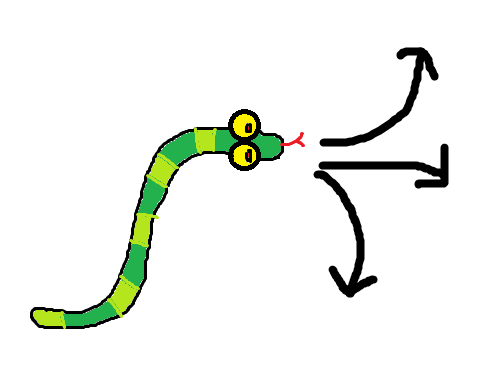
\includegraphics[scale=0.4]{ular-segala-arah}  
	\caption[Pergerakan ular ke segala arah]{Pergerakan ular ke segala arah} 
	\label{fig:ularSegalaArah} 
\end{figure} 

Permainan \textit{Snake} ini dapat dimainkan secara \textit{singleplayer} atau \textit{multiplayer}. \textit{Singleplayer game} adalah permainan yang dapat dimainkan oleh 1 pemain. \textit{Multiplayer game} adalah permainan yang dapat dimainkan oleh beberapa pemain. Permainan \textit{Snake} sekarang dimainkan secara \textit{singleplayer}. Contoh \textit{singleplayer game Snake} adalah \textit{Snake} pada telepon genggam \textit{Nokia} yang dapat dilihat pada Gambar~\ref{fig:nokiaSnake}\footnote{https://en.wikipedia.org/wiki/Snake\_(video\_ game\_ genre)} dan contoh \textit{multiplayer game Snake} adalah \textit{Slither.io} yang dapat dilihat Gambar~\ref{fig:slither}\footnote{https://play.google.com/store/apps/details?id=air.com.hypah.io.slither}. \textit{Snake} dapat dimainkan menggunakan \textit{smartphone} dan \textit{web browser}.  

\begin{figure}[H]
	\centering  
	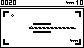
\includegraphics[scale=2]{nokiaSnake}  
	\caption[Permainan Snake pada telepon genggam \textit{Nokia}]{Permainan Snake pada telepon genggam \textit{Nokia}} 
	\label{fig:nokiaSnake} 
\end{figure} 

\begin{figure}[H]
	\centering  
	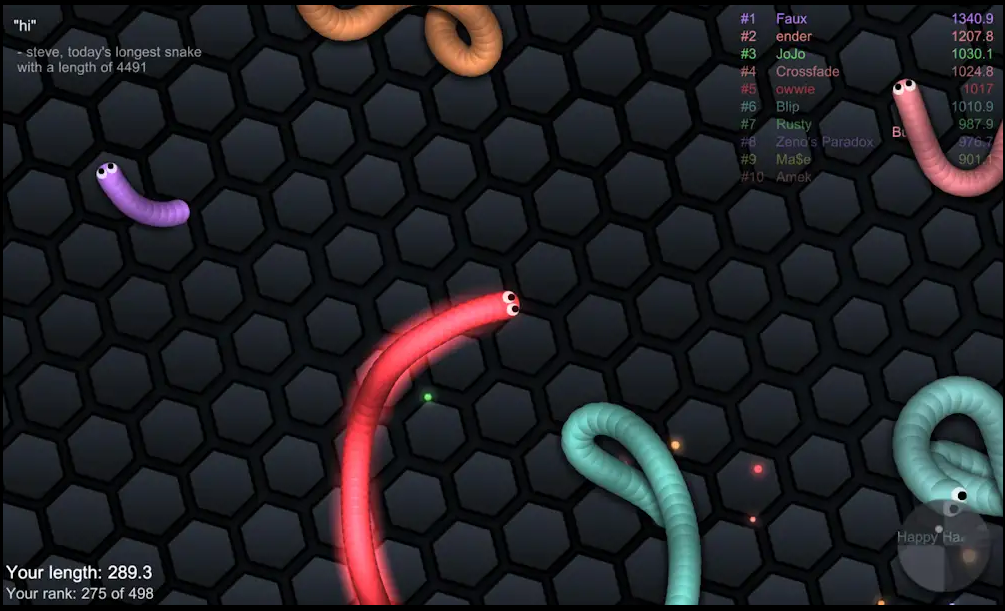
\includegraphics[scale=0.3]{slither}  
	\caption[Permainan \textit{Slither.io} pada \textit{Android}]{Permainan \textit{Slither.io} pada \textit{Android}} 
	\label{fig:slither} 
\end{figure} 

\subsection{HTML5 Canvas}
HTML(\textit{Hyper Text Markup Language}) adalah bahasa markah yang digunakan untuk membuat halaman web. Untuk mengisi konten/isi dari halaman web, digunakan \textit{tag}. HTML5(\textit{Hyper Text Markup Language 5}) adalah versi HTML terbaru yang merupakan penerus dari HTML4, XHTML1, dan DOM \textit{level 2} HTML. HTML5 memiliki beberapa elemen baru, salah satunya yaitu HTML5 Canvas\footnote{https://en.wikipedia.org/wiki/HTML5}. HTML5 Canvas adalah sebuah tempat untuk menggambar \textit{pixel-pixel} yang ditulis menggunakan \textit{Javascript}. HTML5 Canvas API(\textit{Application Programming Interface}) yang paling umum digunakan adalah \textit{2D Context}. \textit{2D Context} ini digunakan untuk membuat bentuk 2 dimensi, menampilkan gambar, membuat tulisan, menambahkan warna, dan membuat garis dan kurva. HTML5 Canvas tidak hanya sekedar untuk membuat bentuk dan menampilkan gambar saja, HTML5 Canvas dapat digunakan untuk membuat animasi, aplikasi web dan \textit{games}. Untuk menambah canvas pada halaman HTML, tambahkan \textit{tag} <canvas> pada \textit{body} HTML seperti pada Gambar~\ref{fig:canvasCode}.

\begin{figure}[H]
	\centering  
	\includegraphics[scale=1]{canvasCode}  
	\caption[Membuat canvas]{Membuat canvas} 
	\label{fig:canvasCode} 
\end{figure} 

Pada Gambar~\ref{fig:canvasCode}, terdapat 3 atribut pada canvas. Berikut adalah penjelasan dari setiap atribut: 
\begin{itemize}
	\item \textit{id}: \textit{id} digunakan sebagai penanda yang akan digunakan oleh \textit{Javascript}. Id dari canvas adalah \textit{snake}.
	\item \textit{Width}: \textit{Width} adalah lebar canvas tersebut. Lebar dari canvas adalah 1340 \textit{pixel}.
	\item \textit{Height}: \textit{Height} adalah tinggi dari canvas tersebut. Tinggi dari canvas adalah 550 \textit{pixel}.
\end{itemize}

\subsection{Javascript dan jQuery}
\textit{Javascript} adalah bahasa pemrograman tingkat tinggi dan merupakan bagian utama dalam pembuatan halaman web selain HTML(\textit{Hyper Text Markup Language}) dan CSS(\textit{Cascading Style Sheet}). \textit{Javascript} membuat halaman web menjadi lebih interaktif. Karena itu, dalam pembuatan halaman web, \textit{Javascript} selalu digunakan. Misalnya ketika pengunjung \textit{website} menekan tombol, maka akan muncul gambar atau tulisan. Kode \textit{Javascript} dituliskan di dalam tag <script> pada HTML. Sintaks \textit{Javascript} hampir mirip dengan bahasa pemrograman Java. Perbedaan yang cukup mencolok adalah \textit{Javascript} dapat menampung tipe data apa saja tanpa mendefinisikan tipe data tersebut pada variabel. Gunakan \textit{'var'} untuk mendeklarasi variabel pada \textit{Javascript}. \\

\textit{jQuery} adalah \textit{library} dari \textit{Javascript} untuk menyederhanakan \textit{script} pada HTML\footnote{https://id.wikipedia.org/wiki/JQuery}. Penulisan menggunakan \textit{jQuery} lebih pendek dibandingkan \textit{Javascript}. \textit{jQuery} membutuhkan sumber \textit{library}. \textit{Library} tersebut dapat disimpan secara internal(di file komputer) atau menggunakan CDN(\textit{Content Delivery Network}). Sintaks pada \textit{jQuery} adalah sebagai berikut:

\begin{displaymath}
	\$(selector).action()\footnote{https://www.w3schools.com/jquery/jquery\_ syntax.asp};
\end{displaymath}

Penjelasan dari sintaks tersebut adalah sebagai berikut: 
\begin{itemize}
	\item Simbol \$ : untuk mengakses \textit{jQuery}.
	\item \textit{Selector} : untuk menemukan elemen HTML. Selector yang biasa digunakan adalah \textit{selector} id(\#) dan \textit{selector class}(.).
	\item \textit{Action} : hal yang akan dilakukan oleh \textit{selector}.
\end{itemize}

Semua \textit{method} pada \textit{jQuery} dituliskan di dalam \textit{document ready event}. \textit{Document ready event} mencegah kode \textit{jQuery} tersebut dieksekusi terlebih dahulu sebelum dokumen sudah siap\footnote{https://www.w3schools.com/jquery/jquery\_ syntax.asp}. Cara penulisanya terdapat pada Gambar~\ref{fig:ready}.

\begin{figure}[H]
	\centering  
	\includegraphics[scale=1]{ready}  
	\caption[\textit{Document ready event}]{\textit{Document ready event}} 
	\label{fig:ready} 
\end{figure} 

\subsubsection{Inisialisasi dan Menggambar pada Canvas}
Sesudah menuliskan \textit{tag} <canvas> pada HTML, canvas tidak bisa langsung digambar. Sebelum menggambar pada canvas, perlu dilakukan inisialisasi menggunakan \textit{Javascript}. Berikut adalah cara menginisialisasi canvas menggunakan \textit{Javascript} pada Gambar~\ref{fig:canvasJS} dan \textit{jQuery} pada Gambar~\ref{fig:canvasJQ}.

\begin{figure}[H]
	\centering
	\caption[Inisialisasi menggunakan \textit{Javascript}]{Inisialisasi menggunakan \textit{Javascript}}
	\centering
	\includegraphics[scale=1]{canvasJS}
	\label{fig:canvasJS} 
\end{figure}

\begin{figure}[H]
	\centering
	\caption[Inisialisasi menggunakan \textit{jQuery}]{Inisialisasi menggunakan \textit{jQuery}}
	\includegraphics[scale=1]{canvasJQ}
	\label{fig:canvasJQ} 
\end{figure}

Sesudah inisialisasi canvas, canvas tersebut dapat digambar dengan bentuk 2D, garis, kurva dan membuat tulisan. Selain untuk menggambar, bentuk-bentuk tersebut dapat diberi warna sesuai dengan keinginan. Berikut adalah perintah untuk membuat bentuk-bentuk 2D: 

\begin{itemize}
	\item \textit{fillRect()} : menggambar sekaligus mewarnai persegi.
	\item \textit{strokeRect()} : menggambar sebuah persegi.
	\item \textit{arc()} : menggambar lingkaran.
\end{itemize}


\subsubsection{Membuat Objek beserta Atribut dan Methodnya}
\textit{Javascript} mendukung OOP(\textit{Object Oriented Programming}) sehingga \textit{programmer} lebih mudah mengerti cara kerja program tersebut. \textit{Object Oriented Programming} merupakan paradigma pemrograman berdasarkan konsep objek\footnote{https://id.wikipedia.org/wiki/Pemrograman\_ berorientasi\_ objek}. Objek tersebut dapat berupa benda-benda yang ada pada kehidupan sehari-hari. Setiap objek memiliki atribut dan \textit{method}. Atribut adalah data dan karakteristik yang terdapat pada objek. \textit{Method} adalah hal yang dapat dilakukan oleh objek tersebut. Contohnya, objek mobil memiliki atribut warna mobil, merk mobil, dan berat mobil. \textit{Method} objek mobil adalah dapat berbelok, dapat berhenti dan dapat maju. \\

Pada \textit{Javascript} untuk membuat objek, digunakan perintah \textit{function}. Pada Gambar~\ref{fig:objectFunctionCode} adalah potongan kode untuk membuat objek pada \textit{Javascript} dengan atribut dan \textit{method}.

\begin{figure}[H]
	\centering  
	\includegraphics[scale=1]{objectFunctionCode}
	\caption[Membuat objek pada \textit{Javascript}]{Membuat objek pada \textit{Javascript}}
	\label{fig:objectFunctionCode} 
\end{figure} 

Berdasarkan potongan kode pada Gambar~\ref{fig:objectFunctionCode}, objek mobil tersebut memiliki atribut yaitu merk mobil, warna mobil dan berat mobil. \textit{Method} dari objek mobil adalah mobil dapat berbelok ke kanan dan ke kiri.

\subsubsection{Events}
\textit{Event} adalah sebuah cara untuk membuat halaman web menjadi lebih interaktif. Javascript akan menjalankan suatu hal apabila \textit{event} tersebut terdeteksi\footnote{https://www.w3schools.com/js/js\_ events.asp}. Misalnya apabila sebuah tombol ditekan pada \textit{web browser}, maka akan muncul tanggal hari ini.  Pada skripsi ini, event yang digunakan adalah event milik \textit{jQuery} dan \textit{event keyboard} akan digunakan. Setiap tombol pada \textit{keyboard} memiliki kode unik/\textit{key code} tersendiri. \textit{Event-event} yang digunakan adalah sebagai berikut:

\begin{itemize}
	\item \textit{keydown} : fungsi akan dieksekusi apabila pengguna menekan sebuah tombol.
	\item \textit{keyup} : fungsi akan dieksekusi apabila pengguna sedang tidak menekan sebuah tombol.
\end{itemize}

Kode-kode pada \textit{keyboard} yang digunakan adalah tombol atas, bawah, kanan dan kiri. Pada Gambar~\ref{fig:eventKeyDown} adalah potongan kode untuk membuat \textit{event keydown}.

\begin{figure}[H]
	\centering  
	\includegraphics[scale=1]{eventKeydown}
	\caption[\textit{Event keydown} pada tombol atas, bawah, kiri, dan kanan]{\textit{Event keydown} pada tombol atas, bawah, kiri, dan kanan}
	\label{fig:eventKeyDown} 
\end{figure} 

\subsubsection{Membuat Animasi}
\textit{Javascript} dan \textit{jQuery} dapat digunakan untuk membuat animasi. Animasi adalah proses pergantian gambar yang hampir berbeda satu dengan yang lainya secara cepat sehingga gambar tersebut seolah-olah bergerak\footnote{https://en.wikipedia.org/wiki/Animation}. Langkah-langkah untuk membuat animasi menggunakan canvas adalah :

\begin{itemize}
	\item \textit{Draw} : gambar objek tersebut
	\item \textit{Update} : \textit{update} posisi dari objek tersebut.
	\item \textit{Clear} : hapus semua objek yang ada pada canvas.
	\item \textit{Repeat} : lakukan 3 hal diatas secara berulang.
\end{itemize}

Untuk membuat animasi, membutuhkan perintah \textit{setTimeout}. \textit{setTimeout} dapat membatasi \textit{framerate} sehingga animasi tidak bergerak terlalu cepat. Sintaks untuk \textit{setTimeout} adalah setTimeout(x,y), di mana x adalah sebuah fungsi yang ingin dibuat animasi dan y adalah \textit{framerate} dari animasi tersebut. Gambar~\ref{fig:animate} menunjukan cara untuk membuat animasi. Fungsi \textit{animate()} di baris paling akhir harus dipanggil lagi supaya animasi dapat berjalan terus-menerus.

\begin{figure}[H]
	\centering  
	\includegraphics[scale=1]{animate}
	\caption[Membuat kotak berpindah posisi]{Membuat kotak berpindah posisi}
	\label{fig:animate} 
\end{figure} 

\subsection{Github}
\textit{Github} adalah layanan \textit{web hosting} bersama untuk proyek pengembangan perangkat lunak yang menggunakan sistem \textit{version control} yaitu \textit{Git}\footnote{https://en.wikipedia.org/wiki/GitHub}. \textit{Git} dapat mengetahui perubahan pada file di komputer. \textit{Github} biasanya digunakan oleh para \textit{programmer} untuk menambahkan/merevisi \textit{source code} dan sebagai media untuk berkolaborasi dalam proyek pembangunan perangkat lunak. \textit{Source code} tersebut disimpan dikelompokan pada file dan file tersebut disimpan di\textit{repository}. Dalam 1 \textit{repository}, \textit{owner}(pengguna yang membuat \textit{repository}) dapat mengundang pengguna lain untuk berkolaborasi. Ketika ada perubahan pada \textit{repository}, maka \textit{collaborator}(pengguna yang diberi hak untuk mengubah \textit{repository}) dapat mengetahui \textit{source code} atau file yang direvisi oleh \textit{collaborator} lain.\\

\textit{Github} memiliki banyak fitur untuk memudahkan kerja \textit{programmer}. Fitur \textit{Github} yang mendukung penelitian ini adalah \textit{pull request}. \textit{Pull request} memberitahu \textit{collaborator} lain tentang perubahan pada \textit{repository}. Dengan adanya \textit{pull request}, pengguna dan \textit{collaborator} lain dapat berdiskusi tentang perubahan tersebut. Perubahan tersebut harus di \textit{merge} oleh \textit{collaborator} dari \textit{repository}. Apabila sudah di \textit{merge} oleh \textit{collaborator}, perubahan tersebut akan disimpan di \textit{repository}\footnote{https://help.github.com/articles/about-pull-requests}.

\section{\LaTeX}
\label{sec:latex}

Mengapa menggunakan \LaTeX{} untuk buku skripsi dan apa keunggulan/kerugiannya bagi mahasiswa dan pembuat template. 

\dtext{13-14}


\section{Template Skripsi FTIS UNPAR}
\label{sec:template}
 
Akan dipaparkan bagaimana menggunakan template ini, termasuk petunjuk singkat membuat referensi, gambar dan tabel.
Juga hal-hal lain yang belum terpikir sampai saat ini. 
 
\dtext{15-16}

\subsection{Tabel}  
Berikut adalah contoh pembuatan tabel. 
Penempatan tabel dan gambar secara umum diatur secara otomatis oleh \LaTeX{}, perhatikan contoh di file bab2.tex untuk melihat bagaimana cara memaksa tabel ditempatkan sesuai keinginan kita.

Perhatikan bawa berbeda dengan penempatan judul gambar gambar, keterangan tabel harus diletakkan di atas tabel!!
Lihat Tabel~\ref{tab:contoh1} berikut ini:

\begin{table}[H] %atau h saja untuk "kira kira di sini"
	\centering 
	\caption{Tabel contoh}
	\label{tab:contoh1}
	\begin{tabular}{cccc}
		\toprule
		& $v_{start}$ & $\mathcal{S}_{1}$ & $v_{end}$\\

		\midrule
		$\tau_{1}$ & 1 & 12& 20\\
		$\tau_{2}$ & 1 &  & 20\\
		$\tau_{3}$ & 1 & 9 & 20\\
		$\tau_{4}$ & 1 &  & 20\\

		\bottomrule
		
	\end{tabular} 
\end{table}
Tabel~\ref{tab:cthwarna1} dan Tabel~\ref{tab:cthwarna2} berikut ini adalah tabel dengan sel yang berwarna dan ada dua tabel yang bersebelahan. 
\begin{table}[H]
	\begin{minipage}[c]{0.49\linewidth}
		\centering
		\caption{Tabel bewarna(1)}
		\label{tab:cthwarna1}
		\begin{tabular}{ccccc}
			\toprule
			 & $v_{start}$ & $\mathcal{S}_{2}$ & $\mathcal{S}_{1}$ & $v_{end}$\\
			
			\midrule
			$\tau_{1}$ & 1 & 5 \cellcolor{green}& 12& 20\\
			$\tau_{2}$ & 1 & 8 \cellcolor{green}& & 20\\
			$\tau_{3}$ & 1 & 2/8/17 \cellcolor{green}& 9 & 20\\
			$\tau_{4}$ & 1 & \cellcolor{red}& & 20\\
			
			\bottomrule

		\end{tabular}
	\end{minipage}
	\begin{minipage}[c]{0.49\linewidth}
		
		\centering 
		\caption{Tabel bewarna(2)}
		\label{tab:cthwarna2}
		\begin{tabular}{ccccc}
			\toprule
			 & $v_{start}$ & $\mathcal{S}_{1}$ & $\mathcal{S}_{2}$ & $v_{end}$\\
			
			\midrule
			$\tau_{1}$ & 1 & 12& 5 \cellcolor{red} &20\\
			$\tau_{2}$ & 1 &  &  8 \cellcolor{green} &20\\
			$\tau_{3}$ & 1 & 9 & 2/8/17 \cellcolor{green} &20\\
			$\tau_{4}$ & 1 &   & \cellcolor{red} &20\\
			
			\bottomrule
		
		\end{tabular}
	\end{minipage}
\end{table}

 
\subsection{Kutipan}
\label{subs:kutipan} 
Berikut contoh kutipan dari berbagai sumber, untuk keterangan lebih lengkap, silahkan membaca file referensi.bib yang disediakan juga di template ini.
Contoh kutipan:
\begin{itemize}
	\item Buku:~\cite{berg:08:compgeom} 
	\item Bab dalam buku:~\cite{kreveld:04:GIS}
	\item Artikel dari Jurnal:~\cite{buchin:13:median}
	\item Artikel dari prosiding seminar/konferensi:~\cite{kreveld:11:median}
	\item Skripsi/Thesis/Disertasi:~\cite{lionov:02:animasi}~\cite{wiratma:10:following}~\cite{wiratma:22:later}
	\item Technical/Scientific Report:~\cite{kreveld:07:watertight}
	\item RFC (Request For Comments):~\cite{RFC1654}
	\item Technical Documentation/Technical Manual:~\cite{Z.500}~\cite{unicode:16:stdv9}~\cite{google:16:and7}
	\item Paten:~\cite{webb:12:comm}
	\item Tidak dipublikasikan:~\cite{wiratma:09:median}~\cite{lionov:11:cpoly}
	\item Laman web:~\cite{erickson:03:cgmodel}  
	\item Lain-lain:~\cite{agung:12:tango}
\end{itemize}    
  
\subsection{Gambar}

Pada hampir semua editor, penempatan gambar di dalam dokumen \LaTeX{} tidak dapat dilakukan melalui proses {\it drag and drop}.
Perhatikan contoh pada file bab2.tex untuk melihat bagaimana cara menempatkan gambar.
Beberapa hal yang harus diperhatikan pada saat menempatkan gambar:
\begin{itemize}
	\item Setiap gambar {\bf harus} diacu di dalam teks (gunakan {\it field} {\sc label})
	\item {\it Field} {\sc caption} digunakan untuk teks pengantar pada gambar. Terdapat dua bagian yaitu yang ada di antara tanda $[$ dan $]$ dan yang ada di antara tanda $\{$ dan $\}$. Yang pertama akan muncul di Daftar Gambar, sedangkan yang kedua akan muncul di teks pengantar gambar. Untuk skripsi ini, samakan isi keduanya.
	\item Jenis file yang dapat digunakan sebagai gambar cukup banyak, tetapi yang paling populer adalah tipe {\sc png} (lihat Gambar~\ref{fig:ularpng}), tipe {\sc jpg} (Gambar~\ref{fig:ularjpg}) dan tipe {\sc pdf} (Gambar~\ref{fig:ularpdf})
	\item Besarnya gambar dapat diatur dengan {\it field} {\sc scale}.
	\item Penempatan gambar diatur menggunakan {\it placement specifier} (di antara tanda  $[$ dan $]$ setelah deklarasi gambar.
	Yang umum digunakan adalah {\bf H} untuk menempatkan gambar {\bf sesuai} penempatannya di file .tex atau  {\bf h} yang berarti "kira-kira" di sini. \\
	Jika tidak menggunakan {\it placement specifier}, \LaTeX{} akan menempatkan gambar secara otomatis untuk menghindari bagian kosong pada dokumen anda.
	Walaupun cara ini sangat mudah, hindarkan terjadinya penempatan dua gambar secara berurutan. 	
	\begin{itemize}
		\item Gambar~\ref{fig:ularpng} ditempatkan di bagian atas halaman, walaupun penempatannya dilakukan setelah penulisan 3 paragraf setelah penjelasan ini.
		\item Gambar~\ref{fig:ularjpg} dengan skala 0.5 ditempatkan di antara dua buah paragraf. Perhatikan penulisannya di dalam file bab2.tex!
		\item Gambar~\ref{fig:ularpdf} ditempatkan menggunakan {\it specifier} {\bf h}.
	\end{itemize}
\end{itemize}
 
\dtext{17-18}
\begin{figure} 
	\centering  
	\includegraphics[scale=1]{ular-png}  
	\caption[Gambar {\it Serpentes} dalam format png]{Gambar {\it Serpentes} dalam format png} 
	\label{fig:ularpng} 
\end{figure} 

\dtext{19-20}
\begin{figure}[H]
	\centering  
	\includegraphics[scale=0.5]{ular-jpg}  
	\caption[Ular kecil]{Ular kecil} 
	\label{fig:ularjpg} 
\end{figure} 
\dtext{21-22}

\begin{figure}[ht] 
	\centering  
	\includegraphics[scale=1]{ular-pdf}  
	\caption[ {\it Serpentes} betina]{ {\it Serpentes} jantan} 
	\label{fig:ularpdf} 
\end{figure} 
 
